\documentclass[10pt,xcolor={dvipsnames}]{beamer}

\usetheme{blei}
\usepackage{verbatim}
\usepackage{graphicx}
\usepackage{tikz}
\usetikzlibrary{calc, shapes.geometric}

\usepackage{hyperref}
\hypersetup{
  colorlinks=true,
  linkcolor=blue,
  filecolor=magenta,      
  urlcolor=cyan
}

\newcommand{\codecomment}[1]{{\color{gray}#1\color{black}}}

% \title{}
% \author{Timothé van Meter}
% \date{\today}

\begin{document}

% ---------------------------------------------------
% ---------------------------------------------------

\title{A \textit{gentle} introduction to the\\\vspace{.2cm}\texttt{command-line}}
\author{}
\date{}

\maketitle

\begin{frame}{\texttt{Command-whatnow}?}
  \visible<2-2>{
    \begin{tikzpicture}[remember picture,overlay]
      \node[at=(current page.center)] (img) {
        \includegraphics[keepaspectratio,
        width=0.8\paperwidth]{img/terminal_horror.png}
      };
    \end{tikzpicture}
  }
  \visible<3->{
    {\large\texttt{command-line} or \texttt{terminal}:\\\hspace{30pt}an interface to communicate with the computer\\}
  }

  \visible<4->{
    \vspace{1cm}
    {\large\hspace{0.3cm}Provides a \textit{privileged} access to the computer resources!\\}
  }
  \visible<5->{
    \vspace{1cm}
    {\large\hspace{0.3cm}It is \textit{sooooooo} easy to use with public AI models!}
  }
\end{frame}


\begin{frame}{A \textit{simplified} view}
  \begin{tikzpicture}[remember picture,overlay]
    \visible<2->{
      \node[] at (2.5,0.8) (computer) {
        \includegraphics[keepaspectratio,width=0.3\paperwidth]{img/motherboard.jpg}
      };
      \node[] at ($(computer) + (0,2.3)$) (computerLabel) {\texttt{Computer}};
    }
    \visible<3->{
      \node[] at ($(computer) + (3,-1.5)$) (terminal) {
        \includegraphics[keepaspectratio,width=0.4\paperwidth]{img/terminal_horror.png}
      };      
    }
    \visible<3-8>{
      \node[] at ($(terminal) + (0.5,2.2)$) (terminalLabel) {\texttt{command-line}};
    }
    \visible<9->{
      \node[] at ($(terminal) + (0.7,2.2)$) (terminalLabel) {\Large\texttt{command-line}};
    }
    \visible<5->{
      \node[] at ($(terminal) + (3,-1.5)$) (excell) {
        \includegraphics[keepaspectratio,width=0.4\paperwidth]{img/excell.jpg}
      };
      \node[] at ($(excell) + (1.4,1.8)$) (excellLabel) {\texttt{graphical program}};
    }
    \visible<4-8>{
      \draw[gray, ultra thick, ->] (computerLabel.mid east) to [in=90, out=20] (terminalLabel.north);
    }
    \visible<9->{
      \draw[red, ultra thick, ->] (computerLabel.mid east) to [in=90, out=20] (terminalLabel.north);
    }
    \visible<6->{
      \draw[gray, ultra thick, ->] (terminalLabel.mid east) to [in=90, out=20] (excellLabel.north);
    }
    \visible<7->{
      \draw[gray, ultra thick, ->] (6,-3.3) to [in=270, out=180] (4.5,-2.7);
    }
    \visible<8-8>{
      \draw[gray, ultra thick, ->] (3,-2) to [in=270, out=180] (2,-1.3);
    }
    \visible<9->{
      \draw[red, ultra thick, ->] (3,-2) to [in=270, out=180] (2,-1.3);
    }    
  \end{tikzpicture}
\end{frame}


\begin{frame}{Why bother?}
  \visible<2->{{\large \textbf{Advantages}}
    \vspace{0.5cm}
  }
  \begin{itemize}
    \visible<3->{\item \textbf{Reliability:}\\very stable (since \textit{circa} 1970)\vspace{0.3cm}}
    \visible<4->{\item \textbf{Freedom:}\\not limited by the small subset of options authorised by the graphical program \vspace{0.3cm}}
    \visible<5->{\item \textbf{Speed:}\\faster interface, optimised programs, small memory use \vspace{0.3cm}}
    \visible<6->{\item \textbf{Modularity:}\\Simple building bricks, but they all work together \vspace{0.3cm}}
    \visible<7->{\item \textbf{Universality:}\\The commands work on all \textbf{Linux} versions and on \textbf{Mac} as well!}
  \end{itemize}  
\end{frame}


\begin{frame}{Syntax}
  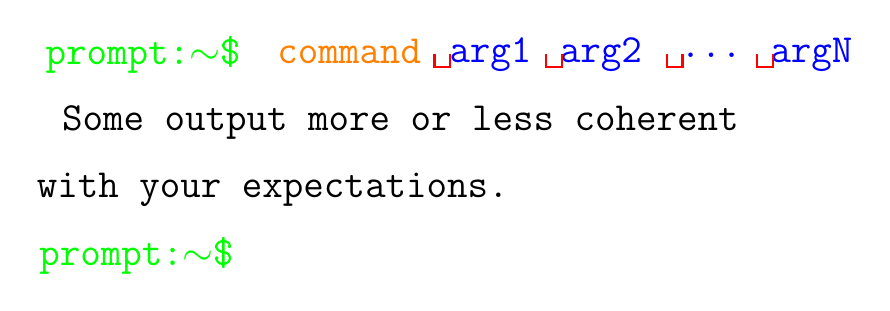
\begin{tikzpicture}[schm/.style={%
      rounded corners,
      thick,
      font = \ttfamily\Large
    }]
    \visible<2->{\node[schm,green] (prompt) at (0,0) {prompt:$\sim$\$};    }
    \visible<3->{\node[schm,orange] (command) at ($(prompt.east) + (1.25,0.05)$) {command};}
    \visible<4->{\node[schm,blue] (arg1) at ($(command.east) + (0.75,-0.05)$) {arg1};}
    \visible<5->{\node[schm,blue] (arg2) at ($(arg1.east) + (0.75,0)$) {arg2};}
    \visible<6->{\node[schm,blue] (punct) at ($(arg2.east) + (0.75,0)$) {...};}
    \visible<7->{\node[schm,blue] (argn) at ($(punct.east) + (0.75,0)$) {argN};}
    \visible<8->{\path[draw, red, thick] (3.7,0.02) -- (3.7,-0.15) -- (3.9,-0.15) -- (3.9,0.02);}
    \visible<9->{\path[draw, red, thick] (5.12,0.02) -- (5.12,-0.15) -- (5.32,-0.15) -- (5.32,0.02);}
    \visible<10->{\path[draw, red, thick] (6.65,0.02) -- (6.65,-0.15) -- (6.85,-0.15) -- (6.85,0.02);}
    \visible<11->{\path[draw, red, thick] (7.8,0.02) -- (7.8,-0.15) -- (8,-0.15) -- (8,0.02);}
    \visible<12->{
      \node[schm] (out) at ($(prompt.south east) + (1.9,-0.5)$) {Some output more or less coherent};
      \node[schm] (out2) at ($(out.south east) + (-6.05,-0.5)$) {with your expectations.};
    }
    \visible<13->{\node[schm,green] (prompt2) at ($(out2.south west) + (1.4,-0.5)$) {prompt:$\sim$\$};}
  \end{tikzpicture}
\end{frame}


\renewcommand\arraystretch{1.5}
\begin{frame}{}
  \begin{center}
    \begin{tabular}{ ccc } 
      COMMAND & ARGUMENTS & DESCRIPTION \\
      \hline
      \hline
      \visible<2->{
      {\large\texttt{pwd}} & none & show the current directory\\
      {\large\texttt{ls}} & possible & show the contents of the location\\
      {\large\texttt{cd}} & always & change the directory location to\\\hline
      }
      \visible<3->{
      {\large\texttt{|}} & always & pipe output to\\
      {\large\texttt{>}} & always & write output to\\
      {\large\texttt{>>}} & always & append output to\\\hline
      }
      \visible<4->{
      {\large\texttt{head}} & always & show the first lines of\\
      {\large\texttt{apropos}} & always & show the commands with the word\\\hline
      }
    \end{tabular}
  \end{center}
\end{frame}


\begin{frame}{Piping \& redirection}
  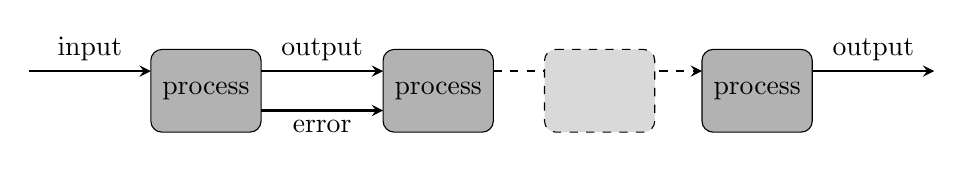
\begin{tikzpicture}[
    proc/.pic={
      % ~~~ back part ~~~~~~~~~~
      \draw [fill=gray!60!, rounded corners] (0,0) -- node[midway,below,yshift=-.3cm] {process} (2,0) -- (2,-1.5) -- (0,-1.5) -- cycle;
    },
    procd/.pic={
      % ~~~ back part ~~~~~~~~~~
      \draw [fill=gray!30!,rounded corners,dashed] (0,0) -- (2,0) -- (2,-1.5) -- (0,-1.5) -- cycle;
    }]    
    \visible<2->{
      \node (p1) at (0,0) {\tikz{\pic [scale=.7] at (0,0) {proc};}};
    }
    \visible<3->{
      \draw[-stealth,thick] (-2.25,0.25) -- node[midway,above] {input} (-0.7,0.25);
      \draw[-stealth,thick] (0.7,0.25) -- node[midway,above] {output} (2.25,0.25);
      \draw[-stealth,thick] (0.7,-0.25) -- node[midway,below] {error} (2.25,-0.25);
    }
    \visible<4->{
      \node (p2) at (2.95,0) {\tikz{\pic [scale=.7] at (0,0) {proc};}};
    }
    \visible<5->{
      \draw[-stealth,thick,dashed] (3.65,0.25) -- (6.3,0.25);
      \node (p3) at (5,0) {\tikz{\pic [scale=.7] at (0,0) {procd};}};
    }
    \visible<6->{
      \node (p4) at (7,0) {\tikz{\pic [scale=.7] at (0,0) {proc};}};
      \draw[-stealth,thick] (7.7,0.25) -- node[midway,above] {output} (9.25,0.25);
    }
  \end{tikzpicture}
\end{frame}


\begin{frame}
  \centering
  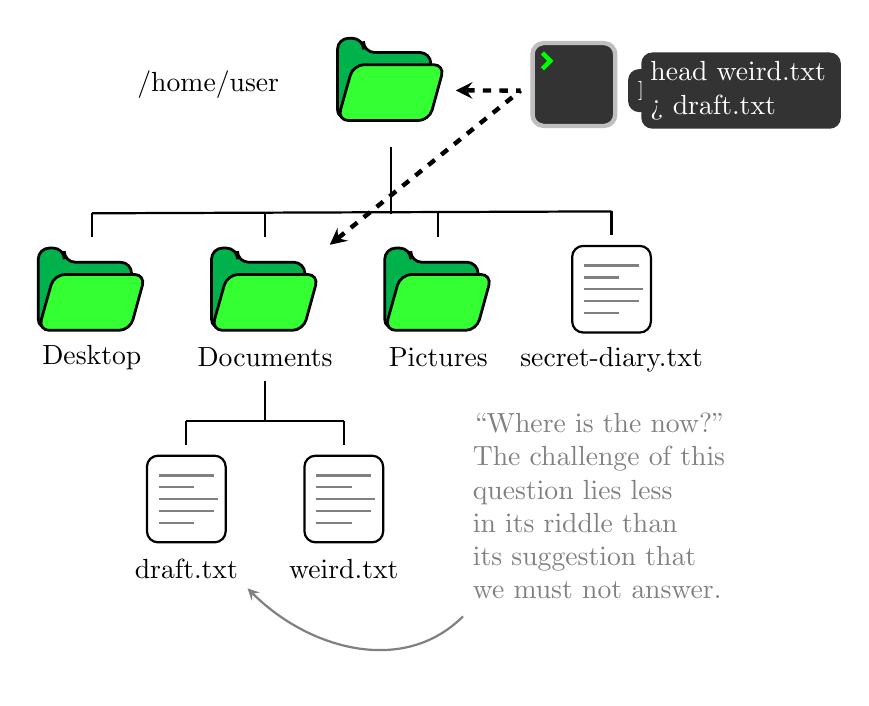
\begin{tikzpicture}[scale=.1,
    % -------------------------------------
    folder/.pic={
      % ~~~ back part ~~~~~~~~~~
      \draw [fill=green!70!blue, rounded corners] (-1.43,-1.05) -- (-1.43,1.04) -- (-0.77,1.04) -- (-0.77,0.68) -- (0.94,0.68) -- (0.94,0.0) -- cycle;
      % ~~~ front part ~~~~~~~~~
      \draw [fill=green!80!, rounded corners] (-1.43,-1.05) -- (-1.03,0.37) -- (1.29,.37) -- (0.90,-1.05) -- cycle;
    },
    terminal/.pic={
      \draw [fill=black!80!] (0,0) -- (1,0) -- (1,-1) -- (0,-1) -- cycle;
      \draw [lightgray,ultra thick,rounded corners] (-0.025,0.025) -- (1.025,0.025) -- (1.025,-1.025) -- (-0.025,-1.025) -- cycle;
      \draw [green,ultra thick] (0.1,-0.1) -- (0.2,-0.2) -- (0.1,-0.3);
    },
    file/.pic={
      \draw [black,thick,rounded corners]  (0,0) -- (2,0) -- (2,-2.2) -- (0,-2.2) -- cycle;
      \draw [gray,thick] (0.3,-0.5) -- (1.7,-0.5);
      \draw [gray,thick] (0.3,-0.8) -- (1.2,-0.8);
      \draw [gray,thick] (0.3,-1.1) -- (1.8,-1.1);
      \draw [gray,thick] (0.3,-1.4) -- (1.7,-1.4);
      \draw [gray,thick] (0.3,-1.7) -- (1.2,-1.7);
    }]
    % -------------------------------------
    % -------------------------------------
    % TOP
    \node (home) at (10,2) {\tikz{\pic [line width=1pt,scale=.5] at (0,0) {folder};}};
    \node (term1) at ($(home.mid east) + (15,4)$) {\tikz\pic at (0,0) {terminal};};
    % -------------------------------------
    % COMMANDS
    \visible<3-4>{\node[fill=black!80!,rounded corners] (pwd) at ($(term1.mid west) + (18,4)$) {\color{white}pwd};}
    \visible<5-6>{\node[fill=black!80!,rounded corners] at ($(term1.mid west) + (18,4)$) {\color{white}ls};}
    \visible<7-8>{\node[fill=black!80!,rounded corners] at ($(term1.mid west) + (26,4)$) {\color{white}cd Documents};}
    \visible<9-10>{\node[fill=black!80!,rounded corners] at ($(term1.mid west) + (18,4)$) {\color{white}ls};}
    \visible<11-12>{\node[fill=black!80!,rounded corners] at ($(term1.mid west) + (26,4)$) {\color{white}head weird.txt};}
    \visible<13->{\node[fill=black!80!,rounded corners,text width=2.3cm] at ($(term1.mid west) + (28,4)$) {\color{white}head weird.txt\\> draft.txt};}
    % -------------------------------------
    % ALL FOLDERS AND FILES
    % -------------------------------------
    \visible<6->{
      \node (desktop) at ($(home.south) + (-38,-20)$) {\tikz{\pic [line width=1pt,scale=.5] at (0,0) {folder};}};
      \node (desktopLabel) at ($(desktop.south) + (0,-2)$) {Desktop};
      % -------------------------------------
      \node (documents) at ($(home.south) + (-16,-20)$) {\tikz{\pic [line width=1pt,scale=.5] at (0,0) {folder};}};
      \node (documentsLabel) at ($(documents.south) + (0,-2)$) {Documents};
      % -------------------------------------
      \node (pictures) at ($(home.south) + (6,-20)$) {\tikz{\pic [line width=1pt,scale=.5] at (0,0) {folder};}};
      \node (picturesLabel) at ($(pictures.south) + (0,-2)$) {Pictures};
      % -------------------------------------
      \node (diary) at ($(home.south) + (28,-20)$) {\tikz{\pic [line width=1pt,scale=.5] at (0,0) {file};}};
      \node (diaryLabel) at ($(diary.south) + (0,-2)$) {secret-diary.txt};
    }
    % -------------------------------------
    \visible<10->{
      \node (weird) at ($(documents.south) + (10,-20)$) {\tikz{\pic [line width=1pt,scale=.5] at (0,0) {file};}};
      \node (weirdLabel) at ($(weird.south) + (0,-2)$) {weird.txt};
      % -------------------------------------
      \node (draft) at ($(documents.south) + (-10,-20)$) {\tikz{\pic [line width=1pt,scale=.5] at (0,0) {file};}};
      \node (draftLabel) at ($(draft.south) + (0,-2)$) {draft.txt};
    }
    % -------------------------------------
    % LINKS
    \visible<6->{
      \draw[-,thick] ($(home.south) + (0,-2)$) -- ($(home.south) + (0,-10.5)$);
      \draw[-,thick] ($(desktop.north) + (0,3)$) -- ($(diary.north) + (0,3)$);
      \draw[-,thick] ($(desktop.north) + (0,3)$) -- ($(desktop.north) + (0,0)$);
      \draw[-,thick] ($(pictures.north) + (0,3)$) -- ($(pictures.north) + (0,0)$);
      \draw[-,thick] ($(diary.north) + (0,3)$) -- ($(diary.north) + (0,0)$);
      \draw[-,thick] ($(documents.north) + (0,3)$) -- ($(documents.north) + (0,0)$);
    }
    \visible<10->{
      \draw[-,thick] ($(documents.south) + (0,-5)$) -- ($(documents.south) + (0,-10)$);
      \draw[-,thick] ($(draft.north) + (0,3)$) -- ($(weird.north) + (0,3)$);
      \draw[-,thick] ($(draft.north) + (0,0)$) -- ($(draft.north) + (0,3)$);
      \draw[-,thick] ($(weird.north) + (0,0)$) -- ($(weird.north) + (0,3)$);
    }
    \visible<2-7>{\draw[stealth-,ultra thick,dashed] ($(home.mid east) + (0,3.25)$) -- ($(term1.mid west) + (0,4)$);}
    \visible<8->{\draw[stealth-,ultra thick,dashed] ($(documents.north east) + (0,-1)$) -- ($(term1.mid west) + (0,4)$);}
    % -------------------------------------
    % OUTPUTS
    \visible<4->{\node (homeLabel) at ($(home.mid west) + (-15,4)$) {/home/user};}
    \visible<12->{\node[gray,text width=4cm] (weirdText) at ($(weird.mid east) + (30,4)$) {``Where is the now?''\\The challenge of this\\question lies less\\in its riddle than\\its suggestion that\\we must not answer.};}
    \visible<14->{\draw[-stealth,thick,gray] ($(weirdText.south west) + (0,-1)$) to[out=225,in=315] ($(draftLabel.south east) + (0,0)$);}
    % -------------------------------------
    % \node[white] at ($(desktop.west) + (-8,0)$) {666};
    % -------------------------------------
  \end{tikzpicture}
\end{frame}


\setbeamercolor{background canvas}{bg=black}
\begin{frame}[t]{\color{red}Some basic commands}
  \vspace{.2cm}
  \visible<+->{\texttt{\color{green} user@computer:$\sim$\$ }}
  \visible<+->{\texttt{\color{white}pwd\\}}
  \visible<+->{\texttt{\color{white}/home/user/\\}}
  \visible<+->{\texttt{\color{green} user@computer:$\sim$\$ }}
  \visible<+->{\texttt{\color{white}ls\\}}
  \visible<+->{\texttt{\color{blue}\textbf{Desktop Documents Pictures} \color{white}secret-diary.txt\\}}
  \visible<+->{\texttt{\color{green} user@computer:$\sim$\$ }}
  \visible<+->{\texttt{\color{white}cd Documents\\}}
  \visible<+->{\texttt{\color{green} user@computer:$\sim$/Documents\$ }}
  \visible<+->{\texttt{\color{white}ls\\}}
  \visible<+->{\texttt{\color{white}weird.txt draft.txt\\}}
  \visible<+->{\texttt{\color{green} user@computer:$\sim$/Documents\$ }}
  \visible<+->{\texttt{\color{white}head }}
  \visible<+->{\texttt{\color{white}weird.txt\\}}
  \visible<+->{\texttt{\color{white}``Where is the now?'' The challenge of this question lies less in its riddle than its suggestion that we must not answer.\\}}
  \visible<+->{\texttt{\color{green} user@computer:$\sim$/Documents\$ }}
  \visible<+->{\texttt{\color{white}head weird.txt}}
  \visible<+->{\texttt{\color{white} > draft.txt\\}}
  \visible<+->{\texttt{\color{green} user@computer:$\sim$/Documents\$ }}
  \visible<+->{\texttt{\color{white}cd ..\\}}
  \visible<+->{\texttt{\color{green} user@computer:$\sim$\$ }}
\end{frame}


% ---------------------------------------------------
% ---------------------------------------------------

\begin{frame}{}
  \thispagestyle{empty}
  \begin{tikzpicture}[remember picture,overlay]
    \node[at=(current page.center)] (img) {
      \includegraphics[keepaspectratio,
      width=1.2\paperwidth]{img/break-time.jpg}
    };
    \node[color=orange] at (6,2) {\Huge \textbf{Time for a break?}};
  \end{tikzpicture}
\end{frame}

% ---------------------------------------------------
% ---------------------------------------------------

\setbeamercolor{background canvas}{bg=white}
\begin{frame}{}
  \centering
  \Large
  \textbf{And now,\\
  Some practical examples}
\end{frame}



\begin{frame}{Example 1: Finding old files}
  \textbf{Problem}:\\
  \vspace{.1cm}
  You want to find a csv dataset which has "musculus" in the name and that was last modified in 1978.\\
  \vspace{.3cm}
  
  \visible<2->{
    \textbf{Solution}:\\
    \vspace{.1cm}
    \texttt{find /home/timothe/ -name "*musculus*.csv"}\\
    \vspace{.3cm}
    \codecomment{Now, let's obtain the date for both files}\\
    \texttt{find /home/timothe/ -name "*musculus*.csv" -ls}\\
  }
\end{frame}


\begin{frame}{Example 2: Renaming files}
  \textbf{Problem}:\\
  \vspace{.1cm}
  Someone miss-labelled samples. They were thinking the DNA was extracted from fox hairs, but indeed they were obtained from a kingfisher. A \textit{very different animal} altogether. There is \textbf{1000 files}. How can we re-label them correctly?\\
  \vspace{.8cm}
  \begin{tikzpicture}
    \visible<2->{
      \node[inner sep=0.5pt,clip,rounded corners=0.6cm] (fox) at (0,0) {
        \includegraphics[width=0.4\paperwidth]{img/vulpes_cropped.jpg}
      };
      \node[] at ($(fox.south) + (0,-0.2)$) {\textit{Vulpes vulpes}};
    }
    \visible<3->{
      \node[inner sep=0.5pt,clip,rounded corners=0.6cm] (kingfisher) at ($(fox) + (7,0)$) {
        \includegraphics[width=0.3\paperwidth]{img/ceyx_cropped.jpg}
      };
      \node[] at ($(kingfisher.south) + (0,-0.2)$) {\textit{Ceyx erithaca}};
    }
    \visible<4->{
      \draw[->, ultra thick] ($(fox.east) + (0.2,0)$) -- node[midway,above] {x $1000$} ($(kingfisher.west) + (-0.2,0)$);
    }
  \end{tikzpicture}
\end{frame}

\begin{frame}{Example 2: Renaming files}
  \textbf{Problem}:\\
  \vspace{.1cm}
  Someone miss-labelled samples. They were thinking the DNA was extracted from fox hairs, but indeed they were obtained from a kingfisher. A \textit{very different animal} altogether. There is \textbf{1000 files}. How can we re-label them correctly?\\
  \vspace{.3cm}
  
  \visible<2->{
    \textbf{Solution}:\\
    \vspace{.1cm}
    \codecomment{Checking that the pattern works:}\\
    \texttt{for i in \$(ls *.fa);\\
      do\\echo \$\{i/Vulpes-vulpes/Ceyx-erithaca\};\\done}\\
    \vspace{.3cm}
    \codecomment{The actual relabelling:}\\
    \texttt{for i in \$(ls *.fa);\\do\\mv \$i \$\{i/Vulpes-vulpes/Ceyx-erithaca\};\\done}
  }
\end{frame}


\begin{frame}{Example 3: Extracting data}
  \textbf{Problem}:\\
  \vspace{.2cm}
  You need to extract from an RNA expression dataset\footnote{Dataset contains consensus transcript expression levels summarized per gene in 51 tissues based on transcriptomics data from HPA and GTEx (data obtained from \href{https://www.proteinatlas.org/humanproteome/tissue/data\#consensus_tissues_rna}{proteinatlas.org}).} all the genes expressed in the heart and order them by decreasing expression (nTPM). Then, save this to a new file called \texttt{heart\_consensus\_rna-decreasing.tsv}.\\
  
  \vspace{1cm}
  \begin{center}
    {\large We have the file, \textit{but how to do it}?}\\
  \end{center}
  
  \vspace{\fill}
\end{frame}



\begin{frame}{Example 3: Solution (part 1)}

\codecomment{Printing the first rows}\\
\texttt{head rna\_tissue\_consensus.tsv}\\
\vspace{0.3cm}
\codecomment{Finding the genes expressed in the heart}\\
\codecomment{First finding the command for the job}\\
\texttt{apropos -a "lines" "pattern" "match"}\\
\vspace{0.3cm}
\codecomment{Finding the corresponding lines in the data}\\
\texttt{grep heart rna\_tissue\_consensus.tsv}\\
\vspace{0.3cm}
\codecomment{The right command}\\
\texttt{apropos -a counts file}\\
\vspace{0.3cm}
\codecomment{How many lines are they?}\\
\texttt{grep heart rna\_tissue\_consensus.tsv | wc -l}\\
\end{frame}

\begin{frame}{Example 3: Solution (part 2)}
\codecomment{Finding out resources for sorting}\\
\texttt{apropos sorting}\\
\vspace{0.3cm}
\codecomment{Sorting the file}\\
\texttt{sort -Vk 5 rna\_tissue\_consensus.tsv}\\
\vspace{0.3cm}
\codecomment{Sorting the file with some visibility}\\
\texttt{sort -Vk 5 rna\_tissue\_consensus.tsv | head}\\
\vspace{0.3cm}
\codecomment{Sorting the file in decreasing order with some visibility}\\
\texttt{sort -rVk 5 rna\_tissue\_consensus.tsv | head}\\
\vspace{0.3cm}
\codecomment{Ordering the heart data}\\
\texttt{grep heart rna\_tissue\_consensus.tsv | sort -rVk 5 | head}\\
\vspace{0.3cm}
\codecomment{Final step, saving the data to a new file}\\
\texttt{grep heart rna\_tissue\_consensus.tsv | \symbol{92}\\
  \hspace{1cm}sort -rVk 5 > heart\_consensus\_rna-decreasing.tsv}\\
\end{frame}



\begin{frame}{Example 4: Using help}
  \only<1>{\textbf{Problem}:\\}\only<2->{\textbf{HARD Problem!}:\\}
  \vspace{.2cm}
  You need to obtain the average value for each gene in multiple tsv files containing two columns: a gene\_id and an expression\_value.

  \vspace{1cm}
  
  \visible<3->{
    \textbf{Solution}:\\
    \vspace{.2cm}
    Ask your favorite LLM, AI prompt for a \texttt{bash} solution!\\
  }
  \visible<4->{
    \vspace{.1cm}
    {\small The minimal query and the bash solution are included in the material.}
  }
  \vspace{\fill}
\end{frame}

\begin{frame}{When to use help?}
  \begin{tikzpicture}
    \node[] (task) at (-0.5,0) {\large\textbf{Long and/or}};
    \node[] at ($(task) + (0,-0.5)$) {\large\textbf{boring task}};
    \draw[] ($(task) + (-1,-1)$) -- ($(task) + (1,-1)$);
    \draw[] ($(task) + (-1,-1.2)$) -- ($(task) + (1,-1.2)$);
    \draw[] ($(task) + (-1,-1.4)$) -- ($(task) + (-0.5,-1.4)$);
    \draw[] ($(task) + (-1,-1.6)$) -- ($(task) + (-0.5,-1.6)$);
    \draw[] ($(task) + (-1,-1.8)$) -- ($(task) + (-0.5,-1.8)$);
    \draw[] ($(task) + (-1,-2)$) -- ($(task) + (-0.2,-2)$);
    \draw[] ($(task) + (-1,-2.2)$) -- ($(task) + (0.7,-2.2)$);
    \draw[] ($(task) + (-1,-2.4)$) -- ($(task) + (0.7,-2.4)$);
    \draw[] ($(task) + (-1,-2.6)$) -- ($(task) + (0.7,-2.6)$);
    \draw[] ($(task) + (-1,-2.8)$) -- ($(task) + (0.5,-2.8)$);
    \draw[] ($(task) + (-1,-3)$) -- ($(task) + (0.5,-3)$);
    \draw[] ($(task) + (-1,-3.2)$) -- ($(task) + (0.5,-3.2)$);
    \draw[] ($(task) + (-1,-3.4)$) -- ($(task) + (0.3,-3.4)$);
    \visible<2->{
      \node[] (think) at ($(task) + (4.5,-0.8)$) {\includegraphics[width=5cm]{binturong.png}};
      \node[draw,ellipse,text width=3.4cm,dashed,thick] (instructions) at ($(think) + (4.8,0)$) {\large \textit{Can you imagine simple instructions for someone else to do it?}};  
      \node[draw,circle,minimum size=0.2cm,dashed,thick] at ($(think) + (1.6,1.2)$) {};
      \node[draw,circle,minimum size=0.2cm,dashed,thick] at ($(think) + (2.4,1)$) {};
    }

    \visible<3->{
      \node[] (ai) at ($(instructions) + (-1,-4)$) {\large \textbf{Query an AI}};
      \path[draw,->,thick] (instructions) --node[midway,right] {\large Yes!} (ai);
    }
    % \visible<4->{
    %   \node[] (text) at ($(ai) + (0.4,-1.2)$) {\textit{How to write the query?}};      
    % }
    \visible<4->{
      \path[draw,->,thick] ($(ai.west) + (0,-0.4)$) to [in=310,out=200] node[midway,below] {\large \textbf{solution \texttt{bash} script}} ($(task) + (0.5,-4)$);
    }
  \end{tikzpicture}  
\end{frame}



\begin{frame}{Online resources}
  Books to learn about and how to use the command-line:\\
  \vspace{.4cm}
  \begin{itemize}
  \item ``Pour aller plus loin avec la ligne de commande``: \href{https://archives.framabook.org/docs/Pour_aller_plus_loin_avec_la_ligne_de_commande/Pour_aller_plus_loin_avec_la_ligne_de_commande_art-libre.pdf}{link}\\
    \vspace{.3cm}
  \item ``COMMAND LINE``: \href{https://static.fsf.org/nosvn/gnu-press/source-files/books/command-line.pdf}{link}\\
    \vspace{.3cm}
  \item ``The Linux Command Line``: \href{https://openlab.citytech.cuny.edu/emt2390l/files/2020/03/The-Linux-Command-Line-Book-5th-Edition.pdf}{link}\\
  \end{itemize}
\end{frame}

\begin{frame}{}
  \begin{center}
    {\Large\textit{All the necessary material and instructions to reproduce\\the examples presented here are available online!}}\\
    \vspace{1.5cm}
    
    \texttt{\href{https://github.com/timothevanmeter/command-line-introduction}{github.com/timothevanmeter/command-line-introduction}}
    \end{center}
  \vspace{1cm}
\end{frame}

\begin{frame}{}
  \centering
  \begin{tikzpicture}[remember picture,overlay]
    \node[] at (current page.center) {\includegraphics[height=\paperheight]{Arctictis_binturong_penicillata.jpg}};
    \node[red] at (0,2.5) {\Huge\textit{Thank you for your attention!}};
  \end{tikzpicture}
\end{frame}


\end{document}
